\begin{ledgroupsized}[r]{120mm}
\footnotesize 
\pstart                
\noindent\textbf{\"{U}berlieferung:}   
\pend
\end{ledgroupsized}
\begin{ledgroupsized}[r]{114mm}
\footnotesize 
\pstart \parindent -6mm
\makebox[6mm][l]{\textit{L}}%
Aufzeichnung: LH XXXVII 5 Bl. 209. 1 Bl. 2\textsuperscript{o}. 1 \unitfrac{1}{4} S. Textträger durch Papiererhaltungs\-maßnahmen gesichert.\\%
Cc 2, Nr. 968 D
\pend
\end{ledgroupsized}
%
\vspace{5mm}
\begin{ledgroup}
\footnotesize 
\pstart
\noindent\footnotesize{\textbf{Datierungsgr\"{u}nde}:
Das vorliegende Stück N. 22 % F/4 = 037,05_209
nimmt ausdrücklich Bezug auf Galileis\protect\index{Namensregister}{\textso{Galilei} (Galilaeus, Galileus), Galileo 1564-1642} Überlegungen über die Bruchfestigkeit von Balken aus dem zweiten Dialog der \textit{Discorsi e dimostrazioni matematiche},
den Leibniz während seines Pariser Aufenthalts in der ersten Ausgabe von Galileis Werken las (\cite{01084}\textit{Opere}, Bologna 1656, Bd. II;
siehe hierüber die Datierungsgründe in N. 19). % F/1 = 037,05_201
N. 22 % F/4 = 037,05_209
knüpft insbesondere an Galileis These an,
dass ein Balken mit parabolischem Profil an jeder Stelle die gleiche Bruchfestigkeit auf\-weise.
Auf dieselbe These spielt ebenfalls das Stück N. 21 % F/3 = 037,05_202-203
an (siehe oben, S. \refpassage{37.05_203r_a1}{37.05_203r_a2}).
Aufgrund dieses inhaltlichen Zusammenhangs wird die Datierung von N. 21 % F/3 = 037,05_202-203
auch für das vorliegende Stück übernommen.}
\pend
\count\Afootins=1200
\count\Bfootins=1000
\count\Cfootins=1000
\end{ledgroup}
%
\vspace{5mm}
\pstart%
\noindent[209~r\textsuperscript{o}]
\pend
\pstart
\normalsize  
% \begin{wrapfigure}{l}{0.5\textwidth}
\vspace{-2mm}
\centering
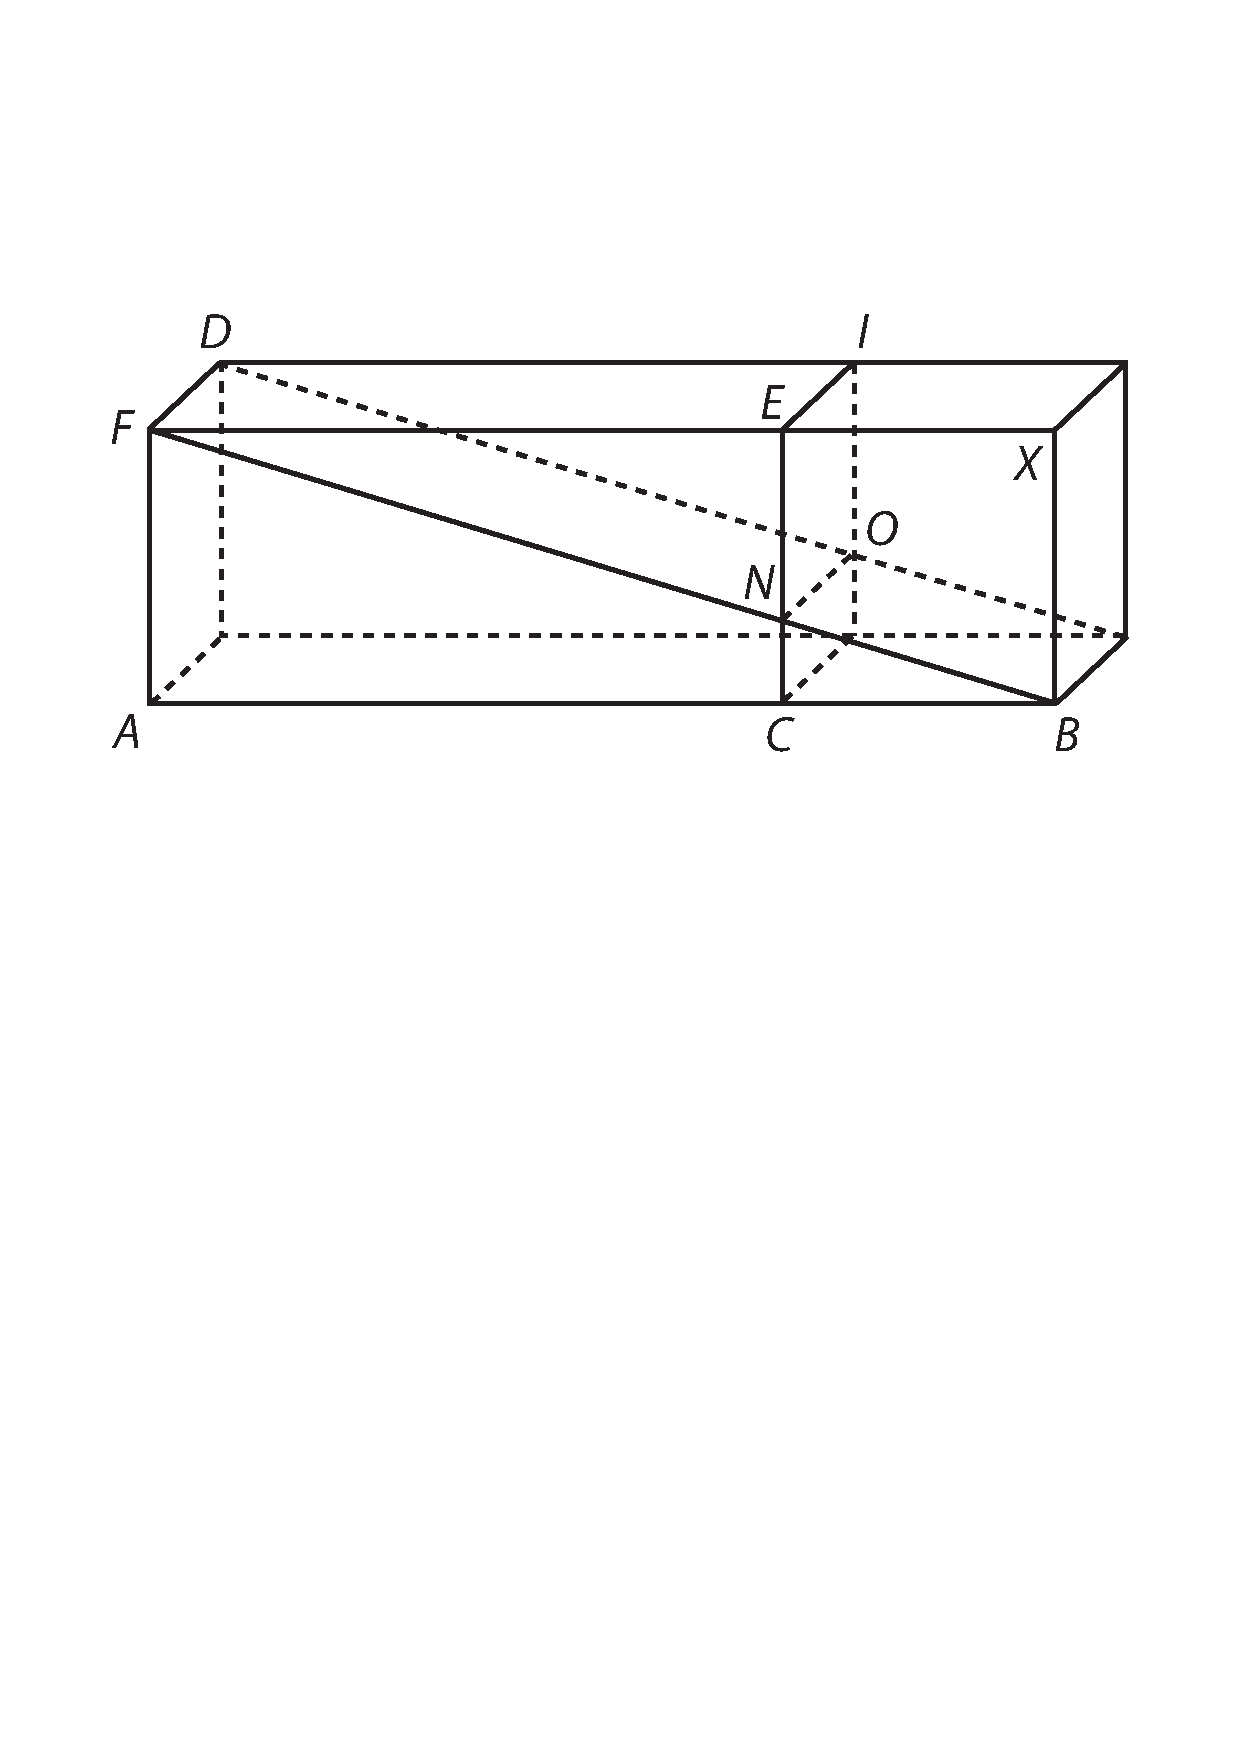
\includegraphics[width=0.54\textwidth]{images/lh03705_209r-d1.pdf}\\
\centering[\textit{Fig. 1}]%
% \end{wrapfigure}
% [209~r\textsuperscript{o}]
\edtext{}{\lemma{\hspace*{1,8mm}[\textit{Fig. 1}]}\killnumber\Cfootnote{Vgl. die Abbildung in \cite{00050}\textsc{G. Galilei}, \textit{Discorsi}, Leiden 1638, S. 138 (\textit{GO} VIII, S. 178).\cite{00048}}}
\pend
\vspace{0.9em}% Rein provisorisch !!!
% \newpage% Rein provisorisch !!!
\pstart
\noindent%
\setline{13}\edtext{Pondera}{\lemma{}\Bfootnote{\textit{(1)} Resistentia\protect\index{Sachverzeichnis}{resistentia} $AF$ ad pondus\protect\index{Sachverzeichnis}{pondus} ex $AB$ est \textit{(2)} Resistentia\protect\index{Sachverzeichnis}{resistentia} in $AF$ contra pondus\protect\index{Sachverzeichnis}{pondus} ex $B$ est ad resistentiam\protect\index{Sachverzeichnis}{resistentia} $CE$ contra \textbar\ idem \textit{erg.} \textbar\ pondus\protect\index{Sachverzeichnis}{pondus} \textit{(a)} ad \textit{(b)} ex $B$ in eadem \textbar\ supposita \textit{erg.} \textbar\ materia resistente, \textit{(aa)} v \textit{(bb)} vel \textit{(cc)} contra \textit{(3)} Pondera \textit{L}}}
\edtext{in $B$}{\lemma{in $B$}\Bfootnote{\textit{erg. L}}}
resistentiis\protect\index{Sachverzeichnis}{resistentia} $AF$ et $CE$ aequivalentia[,]
sunt inter se \edtext{ut lineae suspensionis $CB$ et $AB$ reciproce.}{\lemma{ut}\Bfootnote{\textit{(1)} linea $CB$ ad lineam $AB$ \textit{(2)} lineae [...] reciproce \textit{L}}}
Id ita \edtext{demonstratur. Potentia\protect\index{Sachverzeichnis}{potentia} ponderis pendentis ex $CB$ est ad potentiam ponderis pendentis ex $AC$}{\lemma{demonstratur.}\Bfootnote{\textit{(1)} Resistentiae\protect\index{Sachverzeichnis}{resistentia} $AF$ et $CE$ sunt aequales \textbar\ absolute seu per se spectatae \textit{erg.} \textbar\ : $AF=CE$. \textit{(2)} Pondus pendens ex $CB$ est ad idem pondus ex $AC$ potentiae\protect\index{Sachverzeichnis}{potentia} \textit{(3)} Potentia [...] ex $AC$ \textit{L}}}
in ratione composita ponderum linearumque[,] seu si pondus\protect\index{Sachverzeichnis}{pondus} ex $AB$ sit $l$,
pondus\protect\index{Sachverzeichnis}{pondus} ex $CB$ sit $m$.
illud erit $lAB$, hoc $lCB$.
Erit ergo eorum ratio $lAB \rightpropto [mCB].$\edtext{}{\lemma{$lCB$}\Bfootnote{\textit{L ändert Hrsg.}}}
Jam \edtext{resistentiae\protect\index{Sachverzeichnis}{resistentia} $AF$ et $CE$ sunt aequales,}%
{\lemma{resistentiae}\Bfootnote{%
\textit{(1)} sunt aequale %
\textit{(2)} abso %
\textit{(3)} $AF$ et $CE$ sunt aequales, \textit{L}}}
nempe $AF=CE$.
Ergo et potentiae\protect\index{Sachverzeichnis}{potentia} debent esse aequales.
Ergo $lAB=mCB$.
Ergo si $AB=CB+A$\edtext{[$C$]}{\lemma{$C$}\Bfootnote{\textit{erg. Hrsg.}}}
\edtext{erit $l \lrcorner \llcorner CB+AC \lrcorner =mCB.$}{\lemma{erit}\Bfootnote{%
\textit{(1)} $lAC=$ \textit{(2)} $l \lrcorner \llcorner CB+AC \lrcorner =mCB$ \textit{L}}}
Ergo \protect\rule[-4mm]{0pt}{10mm}$\displaystyle\frac{l}{1}=\displaystyle\frac{mCB}{CB+AC}$.
Ergo $\displaystyle\frac{l}{m}=%
\edtext{%
\displaystyle\frac{CB}{C[B]+AC}.$\edtext{}{\lemma{$B$}\Bfootnote{\textit{erg. Hrsg.}}}
Ergo $\displaystyle\frac{l}{m}=\frac{CB}{AB}$ seu}%
{\lemma{$\displaystyle\frac{CB}{C[B]+AC}.$ Ergo}\Bfootnote{%
\textit{(1)} $lm$ %
\textit{(2)} $\displaystyle\frac{l}{m}=\frac{CB}{AB}$ %
\textit{(a)} Q.E.D. %
\textit{(b)} seu \textit{L}}}
\protect\rule[-4mm]{0pt}{10mm}%
$\displaystyle\efrac{}{\text{ad}}\displaystyle\frac{\text{Pondus ex\ } AB (l)}{\text{Pondus ex\ } CB (m)}$
est reciproce ut $\displaystyle\efrac{\text{linea\ }}{\text{ad lineam\ }}\displaystyle\frac{CB}{AB}.$
\pend
\count\Afootins=1000
\count\Bfootins=1000
\count\Cfootins=1000
\pstart%
\rule[-2,5mm]{0pt}{6mm}%
Quod erat demonstrandum.
\pend
\pstart%
Pondera\protect\index{Sachverzeichnis}{pondus} in $B$
resistentiis\protect\index{Sachverzeichnis}{resistentia} $AF$ et $CN$ aequivalentia sunt inter se
ut lineae suspensionis $CB$ et $AB$ directe.
\pend
\pstart%
Pondera sunto ut ante $l$ et $m$. Linea
\edtext{suspensionis ponderis $l$ esto $AB$, ponderis $m$ esto $CB.$}%
{\lemma{suspensionis ponderis}\Bfootnote{%
\textit{(1)} $l\ AB$ linea %
\textit{(2)} $l$ esto $AB$, ponderis $m$ esto %
\textit{(a)} $CN$ %
\textit{(b)} $CB$ \textit{L}}}
Ergo potentiae
\edtext{$lAB$ et $mCB$. Resistentiae\protect\index{Sachverzeichnis}{resistentia} si ejusdem generis sunt}{\lemma{$lAB$ et}%
\Bfootnote{\textit{(1)} $lCN$ \textit{(2)} $mCB$. \textit{(a)} Ergo resistentiae sunt \textit{(b)} Resistentiae [...] sunt \textit{L}}}
ut quadrata linearum $AF$ et $CN$ seu
\edtext{$AF2 \rightpropto CN2$. Si heterogeneae,}{\lemma{$AF2 \rightpropto CN2.$}\Bfootnote{%
\textit{(1)} Jam potentiae debent esse resisten %
\textit{(2)} Ergo $\displaystyle\frac{AF2}{CN2}=$ %
\textit{(3)} Jam potentiae debent esse resistentiis aequales, ergo %
\textit{(4)} Si heterogeneae, \textit{L}}}
ut diversis lignorum generibus
\edtext{sumtis,}{\lemma{sumtis}\Bfootnote{\textit{erg. L}}}
sunt ex ratione
\edtext{composita ex ratione ipsarum}{\lemma{composita}\Bfootnote{%
\textbar\ ex ratione \textit{erg.} \textbar\ ipsarum \textit{L}}}
resistentiarum,\protect\index{Sachverzeichnis}{resistentia}
\edtext{et ratione quadratorum}{\lemma{et}\Bfootnote{%
\textbar\ ratione \textit{erg.} \textbar\ quadratorum \textit{L}}}
\edtext{seu duplicata}{\lemma{seu duplicata}\Bfootnote{\textit{erg. L}}}
\edtext{linearum. Et}{\lemma{linearum}\Bfootnote{\textit{(1)} seu \textit{(2)} . Et \textit{L}}}
si resistentiae intelligantur in $AF$ esse $n.$ in $CN$ esse $p.$ erunt resistentiae $nAF2$ et $pCN2.$
Quodsi $n=p.$ erunt, ut dixi, ut $AF2 \rightpropto CN2$
\edtext{seu resistentiae erunt: $nAF2$ et $nCN2.$}{\lemma{seu [...] $nCN2$}\Bfootnote{\textit{erg. L}}}
Jam ponderum potentiae\protect\index{Sachverzeichnis}{potentia} aequales esse debent resistentiis\protect\index{Sachverzeichnis}{resistentia}
\edtext{ergo $nAF2=lAB$ et $nCN2=mCB$ et \protect\rule[-4mm]{0pt}{10mm}$\displaystyle\frac{nAF2}{nCN2}=\displaystyle\frac{lAB}{mCB}.$}%
{\lemma{ergo}\Bfootnote{%
\textit{(1)} $\displaystyle\frac{nAF2}{nCN2}=\displaystyle\frac{lAB}{mCB}$ %
\textit{(2)} $nAF2=$ [...] $=\displaystyle\frac{lAB}{mCB}.$ \textit{L}}}
Jam ex figura \protect\rule[-4mm]{0pt}{10mm}$\displaystyle\frac{AB}{CB}=\displaystyle\frac{AF}{CN}$.
\edtext{Ergo dividendo}{\lemma{Ergo}\Bfootnote{\textit{(1)} $nAB2$ \textit{(2)} dividendo \textit{L}}}
utramque rationem, potentiarum et ponderum
per rationem
\rule[-4mm]{0pt}{10mm}%
$\displaystyle\frac{AB}{CB}$ vel $\displaystyle\frac{AF}{CN}$ fiet:
\pend
\newpage
\pstart\noindent%
\rule[-4mm]{0pt}{10mm}
$\displaystyle\frac{nAF}{nCN}=\displaystyle\frac{l}{m}$ vel \rule[-4mm]{0pt}{10mm}$\displaystyle\frac{AF}{CN}=\displaystyle\frac{l}{m}$.
% \rule[-4mm]{0pt}{10mm}
Seu $\displaystyle\efrac{}{\text{ad}}\displaystyle\frac{\text{pondus ex\ } AB (l)}{\text{pondus ex\ } CB (m)}$ est directe ut $\displaystyle\efrac{\text{linea\ }}{\text{ad lineam}}\displaystyle\frac{AF}{CN}=\displaystyle\frac{AB}{CB}$.
%\rule[-3mm]{0pt}{6,5mm}%
Quod erat demonstrandum.
\pend
\pstart%
Quod si vero
\rule[-4mm]{0pt}{10mm}
\edtext{$\displaystyle\frac{AF2}{CN2}=\displaystyle\frac{AC}{CB}.$}{\lemma{$\displaystyle\frac{AF2}{CN2}=$}\Bfootnote{\textit{(1)} $\displaystyle\frac{AC2}{CB2}.$ \textit{(2)} $\displaystyle\frac{AC}{CB}.$ \textit{L}}}
quod fiet si linea $FNB$ sit semiparabolica ex
% \rule[-4mm]{0pt}{10mm}
$\displaystyle\frac{nAF2}{nCN2}=\displaystyle\frac{lAB}{mCB}.$
\rule[-4mm]{0pt}{10mm}%
fiet $\displaystyle\frac{n}{n}=\displaystyle\frac{l}{m}.$
Ergo $l=m.$
Ergo si linea $FNB$ semiparabolica sit, et $B$ vertex[,] pondera in $B$ \edtext{appensa aequivalentia resistentiis\protect\index{Sachverzeichnis}{resistentia} in $AF$ et $CN$ erunt aequalia inter se}{\lemma{appensa}\Bfootnote{\textit{(1)} aequalia erunt ut aequi \textit{(2)} aequivalentia [...] inter se \textit{L}}}.
[209~v\textsuperscript{o}]
\pend
\pstart
Huc usque Galilaeus\protect\index{Namensregister}{\textso{Galilei} (Galilaeus, Galileus), Galileo 1564-1642}
\edtext{lib\edtext{. 2. Dial. Mechan.,}{\lemma{lib. 2. Dial. Mechan.}\Bfootnote{\textit{erg. L}}}%
}{\lemma{lib. 2. Dial. Mechan.}\Cfootnote{Gemeint ist der zweite Dialog in \textsc{G. Galilei}, \textit{Discorsi}, Leiden 1638\cite{00050}, bes. S. 132ff. (\textit{GO} VIII, S. 172ff.)}}
sed qui in applicatione labi visus est:
Dixerat enim
\edtext{%
\textit{E bella cosa sarebbe il ritrovar quale figura devrebbe haver quel tal solido,
che in tutte le sue parti fusse}
[\textit{egualmente}]\edtext{}{\lemma{egalmente}\Bfootnote{\textit{L ändert Hrsg. nach Vorlage}}}
\textit{resistente, tal che non}
\textit{facile fusse ad esser rotto da un peso che lo premesse nel mezzo}
[\textit{più}]\edtext{}{\lemma{piu}\Bfootnote{\textit{L ändert Hrsg. nach Vorlage}}}
\textit{che in qualsivoglia altro luogo.}}{%
\lemma{\textit{E bella} [...] \textit{altro luogo}}\Cfootnote{\cite{00050}a.a.O., S. 137 (\textit{GO} VIII, S. 178).\cite{00048}}}
\pend
\pstart%
Quo facto,
hac quam notis Analyticis nudam exhibui
ratiocinatione usus,
demonstrat de semiparabola\protect\index{Sachverzeichnis}{semiparabola} quae dixi,
atque illi proinde hanc aequalis ubique resistentiae\protect\index{Sachverzeichnis}{resistentia} tribuit praerogativam.
Et
\edtext{
cum\edtext{ notasset}{\lemma{cum}\Bfootnote{\textit{(1)} ostendisset \textit{(2)} notasset \textit{L}}}
figuram semiparabolicam\protect\index{Sachverzeichnis}{semiparabola} $AFNB$ esse ad rectangulum
\edtext{circumscriptum $BAF$}{\lemma{circumscriptum}\Bfootnote{\textit{(1)} $AFI$ \textit{(2)} $BAF$ \textit{L}}}
ut 2 ad 3. subjicit,
\textit{Di quì si vede, come con diminutione di}
\edtext{\textit{peso di} [\textit{più}] \textit{di}}{\lemma{\textit{peso}}\Bfootnote{\textit{di}\ \textbar\ piu \textit{ändert Hrsg. nach Vorlage}\ \textbar\ \textit{(1)} che \textit{(2)} \textit{di} \textit{L}}}
\textit{trenta tré per cento si posson far i travamenti senza diminuir punto la loro gagliardia,
il che ne i Navilii grandi in particolare per regger le coverte può esser d’utile non piccolo;
atteso, che in cotali}
[\textit{fabbriche}]\edtext{}{\lemma{fabriche}\Bfootnote{\textit{L ändert Hrsg. nach Vorlage}}}
\textit{la}
[\textit{leggerezza}]\edtext{}{\lemma{legerezza}\Bfootnote{\textit{L ändert Hrsg. nach Vorlage}}}
\textit{importa infinitamente.}
% \newline%
% \hspace*{7,5mm}%
\textit{Le utilità son tante, che lungo o impossibile sarebbe il registrarle tutte}.}{%
\lemma{cum notasset [...] \textit{registrarle tutte}}\Cfootnote{\cite{00050}a.a.O., S. 141 (\textit{GO} VIII, S. 181).\cite{00048}}}
\pend
\count\Afootins=1500
\count\Bfootins=1500
\count\Cfootins=1500